\documentclass[aspectratio=169]{beamer}
\usepackage{graphicx}
\usepackage{hyperref}
\usetheme{metropolis}
\title{What is a Team?}
\institute{Engineers for Exploration, UC San Diego}
\logo{
\includegraphics[height=.65cm,keepaspectratio]{e4e_logo_350x136.png}}
\setbeamertemplate{caption}[numbered]
\begin{document}
\maketitle
\begin{frame}
    What are some key traits of teams?
\end{frame}
\note[itemize]{
    \item Common Clear Purpose
    \item Good Communication
    \item Respect and Trust
    \item Adaptability
    \item Engagement/Motivation
    \item Psychological Safety
    \item Structure
}
\begin{frame}
    How do we determine the core values of a team?
\end{frame}
\note[itemize]{
    \item This needs to be a consensus between members of the team
    \item Related to the culture of the team
    \item Driven by organizational values and culture
}
\begin{frame}
    What advantages does being on a team bring?
\end{frame}
\note[itemize]{
    \item Different Perspectives/Skills
    \item More manpower
    \item More than the sum of its parts
}
\begin{frame}
    How should teams be structured?
\end{frame}
\note[itemize]{
    \item Flat - individual empowerment
    \item Hierarchical - better focus, clearer structure
    \item And an entire spectrum in between...
}
\begin{frame}{How do teams develop?}
    Every team starts as a group of people
\end{frame}
\begin{frame}{Group Development Cycle}
    \centering
    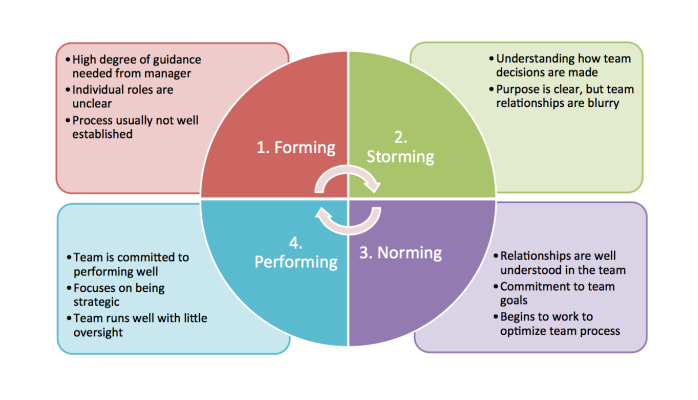
\includegraphics[height=0.8\textheight,width=0.9\textwidth,keepaspectratio]{forming_storming_norming_performing.png} \footnote{\url{https://teambuildingactivity.com/tuckmans-model/}}
\end{frame}
\begin{frame}
    Where do you think your teams are?
\end{frame}
\begin{frame}
    Activity
\end{frame}
\note[itemize]{
    \item Everyone line up in 2 lines
    \item Objective - hold a long rod in place
}
\begin{frame}
    Debrief - how did you do as a team?
\end{frame}
\note[itemize]{
    \item Video Debrief
    \item Focus on the stages of team development
    \item Focus on the resultant structure of the team
    \item Focus on the resultant culture and values of the team
    \item Emphasis - group development needs to be intentionally managed and facilitated
}
\end{document}
